\documentclass[11pt,a4paper]{article}
\usepackage[left=2.5cm,right=2cm, bottom=2cm]{geometry}
\usepackage[utf8]{inputenc}
\usepackage{amsmath}
\usepackage{amsfonts}
\usepackage{amssymb}
\usepackage{amsfonts}
\usepackage{amsmath}
\usepackage{graphicx}
\usepackage{subfigure}
\usepackage{color}
\usepackage{abstract}
\usepackage{float}
\usepackage[toc,page]{appendix}
\usepackage{hyperref}
\usepackage{fancyhdr}
\usepackage{algorithm} 
\usepackage{algpseudocode} 
\usepackage{listings}
\usepackage{xcolor} % for setting colors
% set the default code style
\lstset{
	frame=tb, % draw a frame at the top and bottom of the code block
	tabsize=4, % tab space width
	showstringspaces=false, % don't mark spaces in strings
	numbers=left, % display line numbers on the left
	commentstyle=\color{green}, % comment color
	keywordstyle=\color{blue}, % keyword color
	stringstyle=\color{red} % string color
}

\pagestyle{fancy}
\fancyhf{}
\rhead{\today}
\lhead{\bfseries Alexander Leitner 01525882}
\rfoot{}



\begin{document}
\begin{center}
	\fontsize{24pt}{10pt}\selectfont
	\textsc{\textbf{Computational Science on Many-Core Architectures  Exercise 4}}
\end{center}
\section*{Example 1 Multiple Dot Products (4 Points total)}
\subsection*{a)}
First I tried to implement this with a given $y$-matrix, but it does work that well and I got a SEGMENTATION error.
\begin{lstlisting}[language=C++, caption={kernel for 1a)}]
#include <stdio.h>
# include "timer.hpp"
#include <vector>

__global__ void dot_pro(int N, double *x, double *y0, double *y1, double *y2, 
double *y3, double *y4, double *y5, double *y6, double *y7, double *dot)
{

	unsigned int ind = threadIdx.x + blockDim.x*blockIdx.x;
	unsigned int str = blockDim.x*gridDim.x;

	__shared__ double cache0[256];
	__shared__ double cache1[256];
	__shared__ double cache2[256];
	__shared__ double cache3[256];
	__shared__ double cache4[256];
	__shared__ double cache5[256];
	__shared__ double cache6[256];
	__shared__ double cache7[256];

	double tmpsum0 = 0.0;
	double tmpsum1 = 0.0;
	double tmpsum2 = 0.0;
	double tmpsum3 = 0.0;
	double tmpsum4 = 0.0;
	double tmpsum5 = 0.0;
	double tmpsum6 = 0.0;
	double tmpsum7 = 0.0;

	double val = x[0];

	while(ind < N)
	{
	for (int i = blockIdx.x * blockDim.x + threadIdx.x; i < N; i += blockDim.x * gridDim.x) 
	{
		val = x[i];
		tmpsum0 += val * y0[i];
		tmpsum1 += val * y1[i];
		tmpsum2 += val * y2[i];
		tmpsum3 += val * y3[i];
		tmpsum4 += val * y4[i];
		tmpsum5 += val * y5[i];
		tmpsum6 += val * y6[i];
		tmpsum7 += val * y7[i];
	}
	
	ind += str;
	}

	cache0[threadIdx.x] = tmpsum0;
	cache1[threadIdx.x] = tmpsum1;
	cache2[threadIdx.x] = tmpsum2;
	cache3[threadIdx.x] = tmpsum3;
	cache4[threadIdx.x] = tmpsum4;
	cache5[threadIdx.x] = tmpsum5;
	cache6[threadIdx.x] = tmpsum6;
	cache7[threadIdx.x] = tmpsum7;

	__syncthreads();

	for(int i = blockDim.x/2; i>0; i/=2)
	{
		__syncthreads();
		if(threadIdx.x < i)
		{
			cache0[threadIdx.x] += cache0[threadIdx.x + i];
			cache1[threadIdx.x] += cache1[threadIdx.x + i];
			cache2[threadIdx.x] += cache2[threadIdx.x + i];
			cache3[threadIdx.x] += cache3[threadIdx.x + i];
			cache4[threadIdx.x] += cache4[threadIdx.x + i];
			cache5[threadIdx.x] += cache5[threadIdx.x + i];
			cache6[threadIdx.x] += cache6[threadIdx.x + i];
			cache7[threadIdx.x] += cache7[threadIdx.x + i];
		}
	}

	if(threadIdx.x == 0)
	{
		atomicAdd(dot + 0,cache0[0]);
		atomicAdd(dot + 1,cache1[0]);
		atomicAdd(dot + 2,cache2[0]);
		atomicAdd(dot + 3,cache3[0]);
		atomicAdd(dot + 4,cache4[0]);
		atomicAdd(dot + 5,cache5[0]);
		atomicAdd(dot + 6,cache6[0]);
		atomicAdd(dot + 7,cache7[0]);
	}
}
\end{lstlisting}
\subsection*{b)}
\begin{lstlisting}[language=C++, caption={kernel for 1a)}]
#include <stdio.h>
# include "timer.hpp"
#include <vector>
for (int g = 0; g < anz; g++)
{
	for (int i=0; i<K/8; ++i)
Bandwidth_offset	{
		cudaDeviceSynchronize();
		cudaMemcpy(d_y0, y[i*8+0], sizeof(double)*N, cudaMemcpyHostToDevice);
		cudaMemcpy(d_y1, y[i*8+1], sizeof(double)*N, cudaMemcpyHostToDevice);
		cudaMemcpy(d_y2, y[i*8+2], sizeof(double)*N, cudaMemcpyHostToDevice);
		cudaMemcpy(d_y3, y[i*8+3], sizeof(double)*N, cudaMemcpyHostToDevice);
		cudaMemcpy(d_y4, y[i*8+4], sizeof(double)*N, cudaMemcpyHostToDevice);
		cudaMemcpy(d_y5, y[i*8+5], sizeof(double)*N, cudaMemcpyHostToDevice);
		cudaMemcpy(d_y6, y[i*8+6], sizeof(double)*N, cudaMemcpyHostToDevice);
		cudaMemcpy(d_y7, y[i*8+7], sizeof(double)*N, cudaMemcpyHostToDevice);
		dot_pro<<<s, s>>>(N, d_x, d_y0, d_y1, d_y2, d_y3, d_y4
		, d_y5, d_y6, d_y7, d_res_cblas);
		cudaMemcpy(resultslarge+i*8, d_res_cblas
		, sizeof(double)*8, cudaMemcpyDeviceToHost);
		for (int j = 0; j < 8; j++) 
		{
			res_cblas[j] = 0;
		}
	cudaMemcpy(d_res_cblas, res_cblas, sizeof(double)*8, cudaMemcpyHostToDevice);
	}
}
printf("Dot product took %g seconds", 1000*timer.get()/anz);
\end{lstlisting}
\newpage
\subsection*{c)}
I got a error message that I did not understand and tht's why I could not ran the programm with the other $K$-values.
\begin{figure}[H]
	\centering
	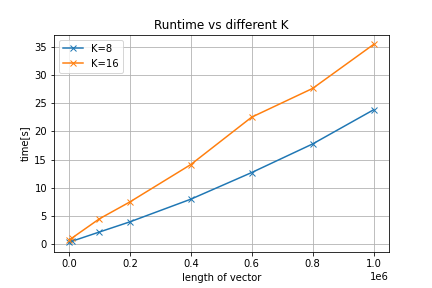
\includegraphics[width=0.5\textwidth]{Bilder/runtime_vs_K}
\end{figure}
\begin{figure}[H]
	\centering
	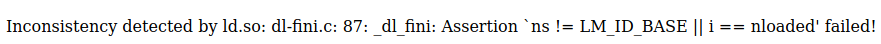
\includegraphics[width=0.7\textwidth]{Error}
\end{figure}
\subsection*{d)}
On approach could be to store the an arbitory number of vectors in a matirx and send it to the kernel and then in kernel calculate the dot-product with a dynamic and static arrays.
\newpage
\section*{Pipelined CG (4 Points total)}
\subsection*{Different Kernels}
\begin{lstlisting}[language=C++, caption={kernel line 7 to 9)}]
 __global__ void x_plus_a_p(int N, double *x, double *p, double *r, double *Ap,
 double alpha, double beta)
{
	for (int i = blockIdx.x * blockDim.x + threadIdx.x; i < N; 
	i += blockDim.x * gridDim.x)
	{
		x[i] = x[i] + alpha * p[i];
		r[i] = r[i] - alpha * Ap[i];
		p[i] = r[i] + beta * p[i];
	}
}
\end{lstlisting}

\begin{lstlisting}[language=C++, caption={kernel line 10 to 12)}]
__global__ void diff_dot_prod(int N, double *Ap, double *p, double *r,
double *ApAp, double *pAp, double *rr, int *csr_rowoffsets, 
int *csr_colindices, double *csr_values)
{
	__shared__ double cache0[512];
	__shared__ double cache1[512];
	__shared__ double cache2[512];
 
	double tmpsum0 = 0;
	double tmpsum1 = 0;
	double tmpsum2 = 0;
 
	for (int i = blockIdx.x * blockDim.x + threadIdx.x; i < N; i += blockDim.x * gridDim.x) 
	{
		double sum = 0;
		for (int k = csr_rowoffsets[i]; k < csr_rowoffsets[i + 1]; k++) 
		{
			sum += csr_values[k] * p[csr_colindices[k]];
		}
		Ap[i] = sum;
	
		tmpsum0 += Ap[i] * Ap[i];
		tmpsum1 += p[i] * Ap[i];
		tmpsum2 += r[i] * r[i];
	}

	cache0[threadIdx.x] = tmpsum0;
	cache1[threadIdx.x] = tmpsum1;
	cache2[threadIdx.x] = tmpsum2;



	for (int k = blockDim.x / 2; k > 0; k /= 2) 
	{
		__syncthreads();
		if (threadIdx.x < k)
		{
			cache0[threadIdx.x] += cache0[threadIdx.x + k];
			cache1[threadIdx.x] += cache1[threadIdx.x + k];
			cache2[threadIdx.x] += cache2[threadIdx.x + k];
		}
	}

	if (threadIdx.x == 0) 
	{
		atomicAdd(ApAp, cache0[0]);
		atomicAdd(pAp, cache1[0]);
		atomicAdd(rr, cache2[0]);
	}
}
\end{lstlisting}

\begin{lstlisting}[language=C++, caption={major loopc for iteration}]
while (1) 
{
	x_plus_a_p<<<512,512>>>(N, cuda_solution, cuda_p, cuda_r, cuda_Ap,
	 alpha, beta);


	cudaMemcpy(cuda_ApAp, &zero, sizeof(double), cudaMemcpyHostToDevice);
	cudaMemcpy(cuda_pAp, &zero, sizeof(double), cudaMemcpyHostToDevice);
	cudaMemcpy(cuda_rr, &zero, sizeof(double), cudaMemcpyHostToDevice);
	diff_dot_prod<<<512,512>>>(N, cuda_Ap, cuda_p, cuda_r, cuda_ApAp,
	 cuda_pAp, cuda_rr, csr_rowoffsets, csr_colindices, csr_values);
	 
	cudaMemcpy(&beta, cuda_ApAp, sizeof(double), cudaMemcpyDeviceToHost);
	cudaMemcpy(&alpha, cuda_pAp, sizeof(double), cudaMemcpyDeviceToHost);
	cudaMemcpy(&residual_norm_squared, cuda_rr, sizeof(double),
	 cudaMemcpyDeviceToHost);


	// line convergence check:
	if (std::sqrt(residual_norm_squared / initial_residual_squared) < 1e-6) 
	{
		break;
	}

	// line 13:
	alpha = residual_norm_squared / alpha;
	
	// line 14:
	beta = alpha * alpha * beta / residual_norm_squared - 1;
	
	if (iters > 10000)
	break; // solver didn't converge
	++iters;
}
\end{lstlisting}

\begin{lstlisting}[language=C++, caption={main}]
for(int i = 100; i < 1200;i = i + 100)
{
	solve_system(i); 
	std::cout << "i:" << i << std::endl;
	std::cout << "" << std::endl;
	std::cout << "" << std::endl;
}
\end{lstlisting}

\subsection*{Benchmark}
\begin{minipage}[t]{0.49\textwidth}
	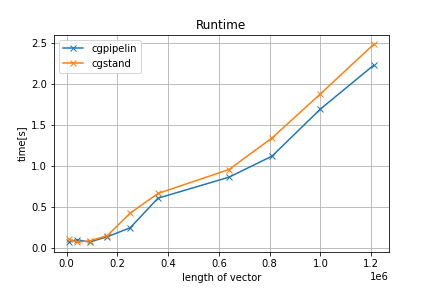
\includegraphics[width=\textwidth]{Bilder/CG_pipelin.png}
\end{minipage}
\begin{minipage}[t]{0.49\textwidth}
	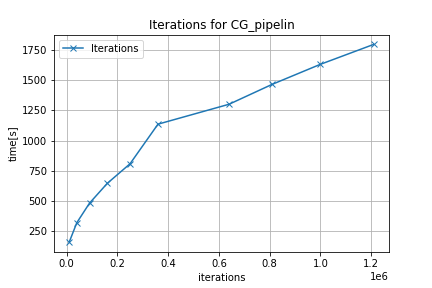
\includegraphics[width=\textwidth]{Bilder/iter.png}
\end{minipage}

\noindent
I expacted that the pipeline CG should perform better and also that the number of iterations should be reduced but the number od iterations are exaktly the same. Maybe I have to wotk on the second kernel in the iteration.
\end{document}